%%%%%%%%%%%%%%%%%%%%%%%%%%%%%%%%%%%%%%%%%
% University/School Laboratory Report
% LaTeX Template
% Version 3.1 (25/3/14)
%
% This template has been downloaded from:
% http://www.LaTeXTemplates.com
%
% Original author:
% Linux and Unix Users Group at Virginia Tech Wiki 
% (https://vtluug.org/wiki/Example_LaTeX_chem_lab_report)
%
% License:
% CC BY-NC-SA 3.0 (http://creativecommons.org/licenses/by-nc-sa/3.0/)
%
%%%%%%%%%%%%%%%%%%%%%%%%%%%%%%%%%%%%%%%%%

%----------------------------------------------------------------------------------------
%	PACKAGES AND DOCUMENT CONFIGURATIONS
%----------------------------------------------------------------------------------------

\documentclass{article}

\usepackage[version=3]{mhchem} % Package for chemical equation typesetting
\usepackage{siunitx} % Provides the \SI{}{} and \si{} command for typesetting SI units
\usepackage{graphicx} % Required for the inclusion of images
\usepackage{natbib} % Required to change bibliography style to APA
\usepackage{amsmath} % Required for some math elements 
\usepackage{float}

\setlength\parindent{0pt} % Removes all indentation from paragraphs

\renewcommand{\labelenumi}{\alph{enumi}.} % Make numbering in the enumerate environment by letter rather than number (e.g. section 6)

%\usepackage{times} % Uncomment to use the Times New Roman font

%----------------------------------------------------------------------------------------
%	DOCUMENT INFORMATION
%----------------------------------------------------------------------------------------

\title{Image Preprocessing\\Gonzalez\\Spatial Preprocessing} % Title

\author{Ahmad \textsc{Asadi}} % Author name

\date{\today} % Date for the report

\begin{document}

\maketitle % Insert the title, author and date

\begin{center}
\begin{tabular}{l r}
Date Performed: & February 21, 2016 \\ % Date the experiment was performed
%Partners: & James Smith \\ % Partner names
%& Mary Smith \\
Instructor: & Professor Safabakhsh % Instructor/supervisor
\end{tabular}
\end{center}

% If you wish to include an abstract, uncomment the lines below
% \begin{abstract}
% Abstract text
% \end{abstract}

%----------------------------------------------------------------------------------------
%	SECTION 1
%----------------------------------------------------------------------------------------

\section{Overview and Definitions}
\begin{description}
\item [Spatial Domain Process] Formally is defined as:\\
	\begin{center}$g(x,y) = T[f(x,y)]$\end{center}
	where $T$ is an operator defined over a neighbourhood of $(x,y)$ on $f$. Also it can be defined on a set of input images.
\item [Definition of Neighbourhood] 
	Usually as a \textbf{square or rectangular subimage} centered at $(x,y)$.
\item [Gray-level transformation] If neighbourhood radius is equal to 1 then $T$ is a \textbf{Gray-level}, or \textbf{Intensity} or \textbf{Mapping}, transformation function.
It is:\\
	\begin{center}$ s = T(r) $\end{center}
	where s and r are respectively the gray level of $g(x,y)$ and $f(x,y)$.\\
	\textbf{Techniques using gray-level transformation, as they operate on just a single point, are mostly referred to as \textit{point processing}.}
\item [Mask] Masks or filters are 2D arrays with a specific size in which inner weights define the application and effect of the mask.
\end{description}

%------------------------------------------------------------------------------------
\section{Some Basic Gray-level Transformations}
 \begin{description}
 \item [Negative Image] A negative image of an input image with gray levels in the range [0 , L-1] is defined as:\\
 \begin{center}
 $s = (L-1) - r$
 \end{center}
 Following is an example of application:
 \begin{figure}[h]
 \center
\makebox[\textwidth]{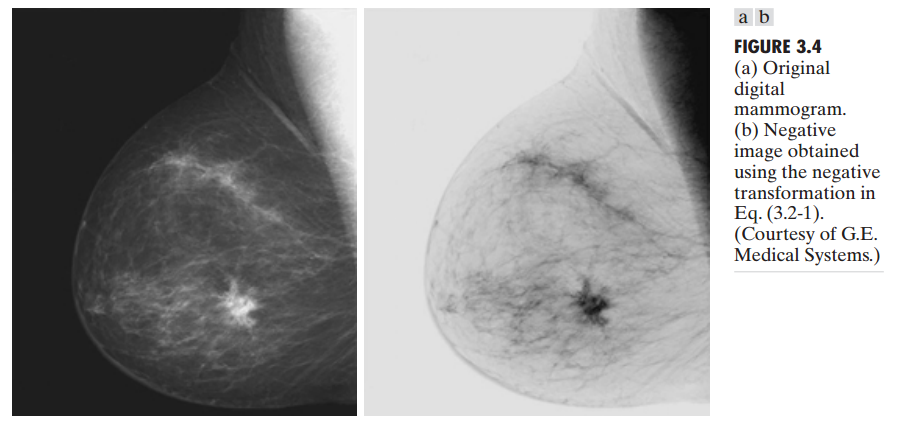
\includegraphics[width=300px]{./Imgs/neg.png}}
\caption{This figure illustrates evident contribution of reversing the intensity (negating image) to illustrate existence of lesion in a part of body.}
 \end{figure}
 
 \item [Log Transformation] The general form of this transformation is as follows:\\
 \begin{center}
 $s = c \log^{(1+r)}$
 \end{center}
 This transformation maps a narrow range of low gray-levels in input image to a wider range in output.\\
 This transformation is appropriate for applications in which having more details of darker parts of image along with bright parts makes worthwhile contributions to accomplish the required task.
 \begin{figure}[h]
 \center
 \makebox[\textwidth]{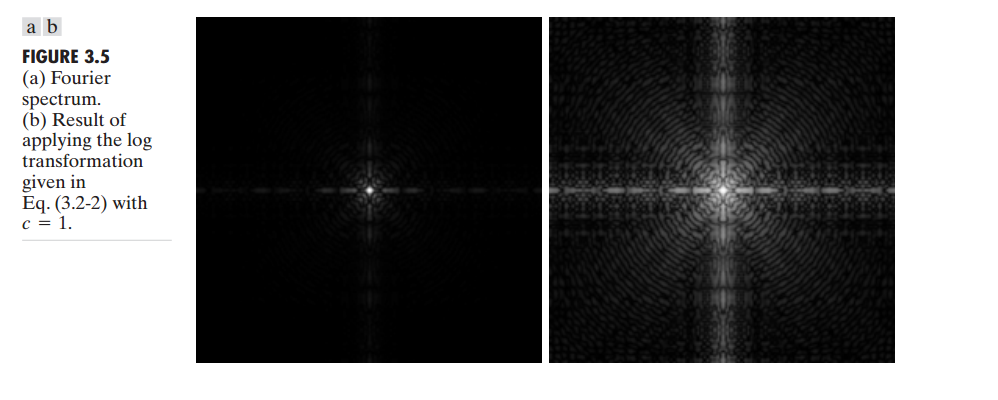
\includegraphics[width=300px]{./Imgs/log.png}}
 \caption{Log transformation effect on input picture}
 \end{figure}
 
 \item [Power-Law Transformation] This kind of transformation has a basic form as follows.\\
\begin{center}
$s = cr^\gamma$
\end{center} 
This transformation is sort of generalization for log-transformation. As it is displayed in fig\ref{fig:powerDiag}, in which plots of $s$ versus $r$ for various
values of $\gamma$ are shown, with lower values of $\gamma$ than 1 this transformation operates as a log-transformation and in cases with $\gamma$ values larger than 1, it operates totally inversely.

\begin{figure}[h]
\center
\makebox[\textwidth]{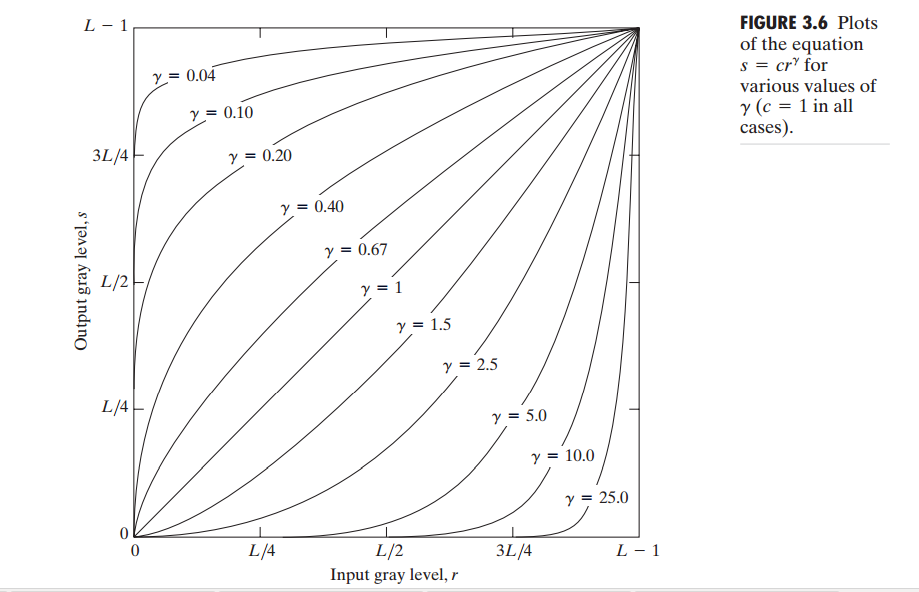
\includegraphics[width=300px]{./Imgs/powerDiag.png}}
\caption{Plots of s versus r for various values of $\gamma$}
\label{fig:powerDiag}
\end{figure}

 One of the most important and useful applications of this transformation is \textbf{gamma correction} in which value ranges in an input image would be mapped to a more appropriate range for certain image displayers to generate fitter images. The value of $\gamma$ in different applications corresponds to the using device and its properties. In fig\ref{fig:gamma0.4} in gamma correction process is $\gamma = 0.4$.\\
 Note that,  varying the value of gamma correction changes not only the brightness, but also the ratios of red to green to blue.\\
 
 \begin{figure}[h]
 \center
 \makebox[\textwidth]{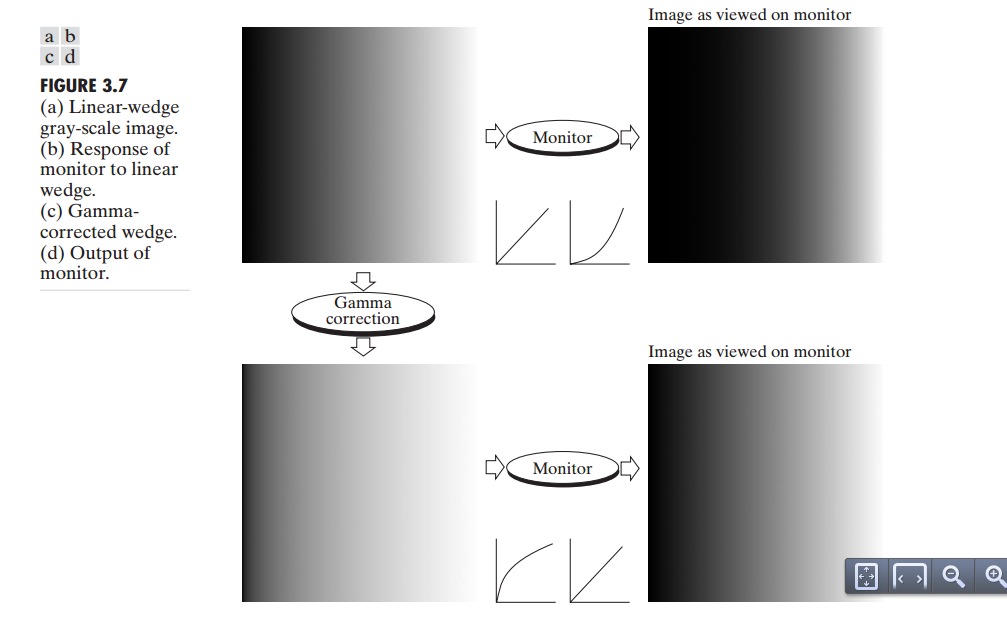
\includegraphics[width = 300px]{./Imgs/powerLaw.png}}
 \caption{Power-Law Transformation result and effect on an input image}
 \label{fig:gamma0.4}
 \end{figure}


 Note that, power-law transformation also affects image's contrast. Fig\ref{fig:powerLawContrast} illustrate the effect of this transformation on image's contrast. In this picture, the value of $\gamma$ increases in each case.
 
 \begin{figure}[h]
 \center
 \makebox[\textwidth]{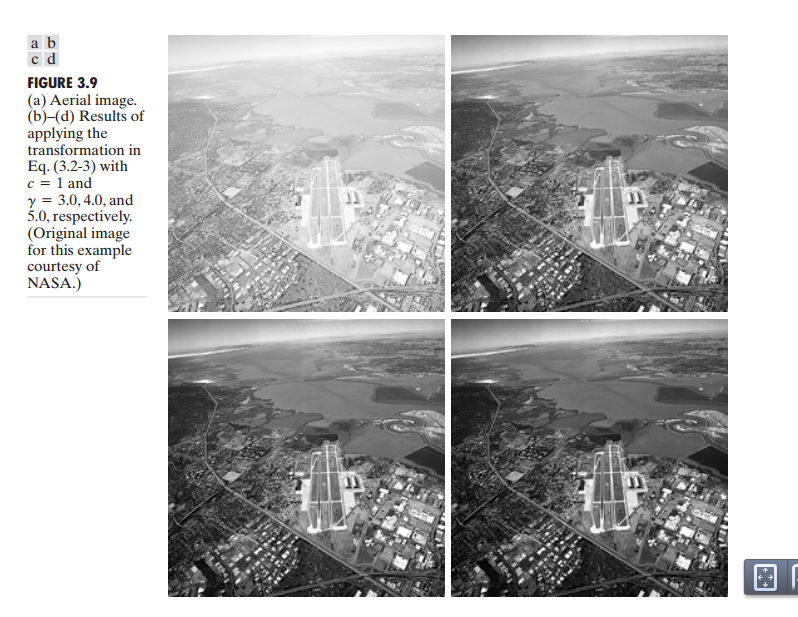
\includegraphics[width=300px]{./Imgs/powerLawContrast.png}}
 \caption{An illustration of power-law transformation's effect on image contrast.}
 \label{fig:powerLawContrast}
 \end{figure}
 
 
 \item [Piecewise-Linear Transformation Functions] This kind of transformation, fragments a transformation range to several subtransformations each specified in a disjoint range of overall transformation's definition range. Thus in each subtransformation any of above-mentioned transformations are applicable. Event though, this method provides us a great opportunity to make more complex and more advantageous transformations, it needs more user input.\\
 There are some examples of this method's applications.
 \begin{description}
 \item [Contrast Stretching] Creating a transformation function which is partially defined for different ranges for $(r,s)$ pairs. Fig\ref{fig:[pieceWiseContrast} demonstrates such an example function.
 \begin{figure}[h]
 \center
 \makebox[\textwidth]{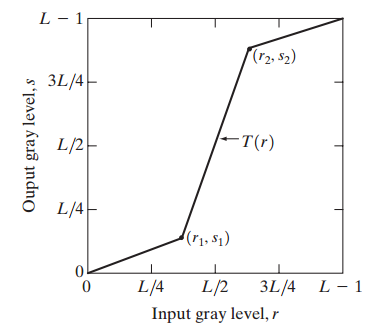
\includegraphics[width=200px]{./Imgs/pieceWiseContrast.png}}
 \caption{An example of piecewise-transformation function for contrast stretching.}
 \label{fig:[pieceWiseContrast}
 \end{figure}
 
 \item[Gray-Level Slicing] This kind of transformation is widely used in making a specified gray-level range of input image more salience. 
 
 \item[Bit-Plane Slicing] Separating bit planes of an image can make worthwhile contribution in achieving better results in applications. Fig\ref{fig:bitPlaneSlicing} displays application of such transformation on an input image of a fractal.
\begin{figure}
\center
\makebox[\textwidth]{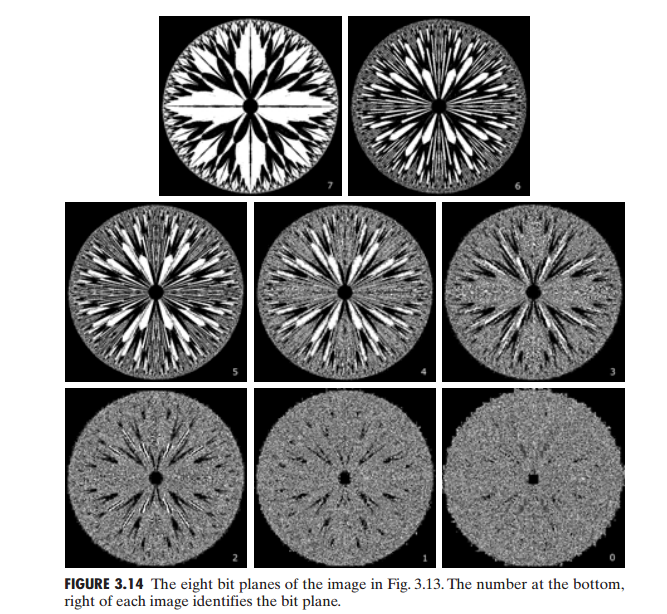
\includegraphics[width=300px]{./Imgs/bitPlaneSlicing.png}}
\caption{Applying a bit-plane slicing transformation on bit planes of a fractal image in order to separate bit-planes.}
\label{fig:bitPlaneSlicing}
\end{figure} 
 
 \end{description}
 
 
 \end{description}
%----------------------------------------------------------------------------------------
%	BIBLIOGRAPHY
%----------------------------------------------------------------------------------------

\bibliographystyle{apalike}

\bibliography{sample}

%----------------------------------------------------------------------------------------


\end{document}